\documentclass[conference]{IEEEtran}
\usepackage{cite}
\usepackage{amsmath,amssymb}
\usepackage{graphicx}
\usepackage{url}
\begin{document}
\title{VeriFuse: Multimodal Image-Text Consistency Classification}
\author{\IEEEauthorblockN{Sanskar Patidar (S24CSEU1513), Dhruv Bhoi (S24CSEU1516), Aishani Mittal (S24CSEU1545)\\Yana Sharma (S24CSEU1523), Nainika Upadhyay (S24CSEU1524)}\IEEEauthorblockA{Bennett University, India\\CSET 346 Project}}
\maketitle
\begin{abstract}
This paper evaluates separate text and image models in two image-text classification settings implemented in VeriFuse. A controlled synthetic benchmark tests whether captions agree with simple colored-shape scenes. A real-media subset from a community mirror of Fakeddit tests prediction of inherited source-community labels. The synthetic text classifier uses train-fitted term frequency-inverse document frequency (TF-IDF) features and logistic regression; the image classifier uses pixel-derived attributes; and feature fusion adds explicit caption-image comparisons. On 144 held-out synthetic pairs, feature fusion reaches 100.0\% accuracy and F1, while text-only and image-only F1 are 47.6\% and 54.8\%. It also reaches 100.0\% on 144 count-manipulation pairs withheld from training. For the real-media subset, the text model uses TF-IDF and logistic regression, while the image model uses frozen CLIP ViT-B/32 image features and a separately fitted logistic classifier. On 1,415 test posts, feature fusion obtains 83.4\% accuracy, 0.645 macro F1, and 0.852 ROC-AUC. These results concern different label definitions and are evaluated separately. Synthetic scores measure controlled consistency; real-media scores predict noisy inherited labels and do not establish factual truth or image authenticity.
\end{abstract}
\begin{IEEEkeywords}
multimodal classification, text classification, image classification, feature fusion, TF-IDF, CLIP, dataset shift
\end{IEEEkeywords}
\section{Introduction}
An image and its accompanying text provide related but distinct evidence. A caption can conflict with visible content, while a social-media post can receive a misleading or satirical source label even when its image is unaltered. A system that combines modalities should therefore be evaluated against a clearly defined target and dataset.

VeriFuse was developed as a reproducible course project with a controlled synthetic task and a later real-media experiment. The synthetic task labels an image-caption pair as REAL when a generated scene matches its caption and FAKE when one visual or textual attribute is changed. It isolates cross-modal consistency but uses a narrow visual grammar. The real-media experiment uses a subset of Fakeddit distributed by a community mirror. Its labels are mapped from source categories and are not independent fact checks.

The project uses modality-specific models in the real-media profile: TF-IDF with logistic regression for text, and frozen CLIP visual representations with a separate logistic classifier for images. The synthetic profile retains its own text model and pixel-attribute image model. The weights are fit independently because the datasets have different label sources and tasks. This paper reports each experiment separately and does not claim that the scores are directly comparable.

The contribution is an implementation and held-out evaluation of these model branches, two fusion strategies per setting, and an account of where each evaluation can support a conclusion. The synthetic experiment tests controlled attribute disagreement. The real-media experiment measures prediction of inherited dataset labels. Neither demonstrates general-purpose deepfake detection.

Three questions guide the evaluation. First, can text-only or image-only features solve the synthetic consistency task when the label is defined by the relation between the modalities? Second, does concatenating modality features improve prediction of the real-media source labels over either branch alone? Third, how does class imbalance change the interpretation of a higher accuracy score? These questions are deliberately scoped to the available data and implementation. They do not ask whether a post is true in the world, whether an author intended to deceive, or whether an image has been edited. The synthetic benchmark is used to isolate a known relation; the mirror dataset is used to test a separate weak-label prediction problem.

The distinction also informs the model comparison. On synthetic scenes, the visual vocabulary and caption vocabulary are both small and the contradictions can be represented as explicit attributes. On real posts, captions are unrestricted and the image content is diverse, so CLIP features are used for visual transfer. The same name for a class does not make the two tasks equivalent: REAL and FAKE have different operational definitions in the two profiles.
\section{Literature Survey}
Fakeddit introduced a multimodal benchmark for fine-grained fake-news classification using Reddit posts and distant supervision from source communities \cite{nakamura}. Source-derived labels are useful for dataset classification, but they are not equivalent to independent verification of each claim. The real-media experiment follows this distinction and reports its label mapping.

CLIP learns image and text representations from large-scale image-caption pairs using contrastive language supervision \cite{radford}. Its visual encoder provides the real-data image representation in VeriFuse. CLIP is frozen in this experiment; only logistic classifier heads are fitted on the local corpus. The text classifier is instead TF-IDF with logistic regression, so the real-data system does not use one shared encoder for both branches.

Image-manipulation research has also studied visual artifacts directly. FaceForensics++ evaluates manipulated facial videos and images under a different task and data regime \cite{rossler}. Its target is not the same as either controlled caption consistency or Fakeddit source-category labels. Its results therefore cannot be inferred from the experiments reported here.

The three references frame different technical questions. Fakeddit provides multimodal social-media records and fine-grained categories, whereas the local real-data profile collapses source categories into two labels for a tractable classification experiment [1]. CLIP provides a transferable visual representation learned from image-text supervision; in VeriFuse, only its image encoder is used and its parameters are frozen [2]. FaceForensics++ focuses on facial manipulation and contains a dedicated manipulation benchmark, so it is relevant as a boundary case for the terminology of authenticity rather than as a directly comparable method [3]. The project does not reproduce those studies or claim their reported performance. The local comparison instead asks whether lightweight, separately trained heads and a feature concatenation improve prediction on the project's own partitions.

These distinctions motivate a conservative use of terms. A source label, an image-caption consistency label, and a forensic manipulation label describe different targets. A system can make a correct prediction for one target and still fail on another. The paper therefore calls its real-media output a prediction of inherited dataset labels and reserves the term consistency for the controlled synthetic task. This avoids treating a broad FAKE category as an annotation that an image itself is forged.

TF-IDF represents documents by term frequency weighted by inverse document frequency, providing a lightweight text baseline \cite{salton}. Logistic regression supplies a linear classifier for these features. VeriFuse uses this baseline on both datasets but fits separate vocabularies and classifiers. Its weak synthetic text-only result illustrates that caption wording alone does not expose the relation between an image and its caption.
\section{Dataset Used}
\subsection{Controlled synthetic benchmark}
The synthetic dataset contains 864 image-caption pairs derived from 432 procedural scenes. Supported objects are red, blue, green, or yellow circles, squares, and triangles, in counts from one to three. Each scene has a matching pair and a paired contradiction created by changing a caption or image attribute. Labels encode this generated consistency rule, not real-world truth.

Groups are separated by source scene. Training contains 432 records from 216 groups; validation and in-distribution test sets contain 144 records each from 72 groups. A separate 144-record test with count manipulations evaluates a held-out contradiction type. The split prevents a scene and its altered counterpart from crossing partitions, although all partitions share the generated visual grammar.

The renderer uses a light background and draws one to three non-overlapping objects, with color and shape selected from the supported set. Each source scene supplies a matching example and an associated mismatch example. The construction balances REAL and FAKE labels in every partition. The mismatch can be introduced through a changed color, shape, or count statement or through a corresponding visual attribute change. Since the generator defines the target, labels are internally consistent by construction; they do not require annotators to judge whether an open-world caption is misleading. Count contradictions are excluded from the ordinary training, validation, and test mismatch patterns and reserved for the separate manipulation test. New scene groups are assigned to that test, so neither the exact base scene nor its paired variant is reused from training.

This design makes the synthetic benchmark useful for controlled checks of feature extraction and fusion, but it also creates a direct relationship between the label-generation rule and the six comparison features used by the fused classifier. Accordingly, perfect held-out performance is evidence that the implementation can recover this constructed rule. It is not an unbiased estimate of performance on natural images, where object boundaries, occlusion, paraphrase, context, and ambiguous captions are substantially more complex.
\subsection{Real-media subset}
The real-media profile uses the \texttt{ams-99/fakeddit\_9k} community mirror \cite{mirror}, pinned at revision \texttt{2ba956a67d2bab34de97b25d71af520ab3fe1e6e}. The import retained 8,585 records after auditing supplied image, text, and source identifiers. Mirror partitions were retained after removing cross-partition overlaps. The mirror does not establish official Fakeddit split provenance; this is a subset evaluation.

Source label 0 (true) maps to REAL and labels 1--5 (satire, false connection, imposter, manipulated, and misleading content) map to FAKE \cite{labelmap}. FAKE therefore combines distinct community categories; it does not mean a post is proven false or that an image was manipulated. Training, validation, and test contain 4,799, 2,371, and 1,415 posts, respectively. The test set has 278 REAL and 1,137 FAKE records, making the labels substantially imbalanced.

The data audit checked the identifiers available in the mirror, including source image and text identifiers, along with supplied exact image and text hashes. It removed 61 rows before retaining the reported 8,585 examples and found no checked cross-partition collision after exclusions. The audit does not establish that related posts about the same event are independent. The mirror lacks original Reddit post identifiers and documented sampling and split provenance; near-duplicate events and overlap with the frozen encoder's pretraining data remain possible. For these reasons, the data are described as a subset evaluation from a community mirror rather than a reproduction of the official benchmark split. The three partitions retain their mirror assignments, and all feature fitting and model selection are constrained to the training and validation partitions.

The test prevalence is 80.4 percent FAKE, compared with 80.4 percent in training and 80.2 percent in validation. Although the proportions are similar, a majority-only prediction can still appear strong under accuracy. The training split contains 941 REAL and 3,858 FAKE posts; validation contains 470 REAL and 1,901 FAKE posts. The held-out test has 278 REAL and 1,137 FAKE posts. These counts are used when interpreting class-specific measures and the majority baseline. They also show why a single aggregate value cannot summarize the system's behavior for both classes.

The dataset is not a balanced sample of verified true and false claims. The combined FAKE class includes several different source categories, and the source's true class is retained as a source annotation rather than independently confirmed ground truth. Thus, the supervised task is to predict the source-derived binary mapping. The evaluation cannot isolate whether a model responds to an image-caption mismatch, a topic, a subreddit convention, or other correlated signals in the posts. The label mapping is documented explicitly to make this target distinction visible.
\begin{table}[t]
\caption{Dataset Partitions}\label{tab:splits}\centering\footnotesize
\begin{tabular}{lrrrr}
\hline Dataset and split & Records & REAL & FAKE & Groups\\\hline
Synthetic train & 432 & 216 & 216 & 216\\
Synthetic validation & 144 & 72 & 72 & 72\\
Synthetic test & 144 & 72 & 72 & 72\\
Synthetic count OOD & 144 & 72 & 72 & 72\\
Real train & 4,799 & 941 & 3,858 & 4,720\\
Real validation & 2,371 & 470 & 1,901 & 2,370\\
Real test & 1,415 & 278 & 1,137 & 1,413\\\hline
\end{tabular}
\end{table}
\section{Proposed Methodology}
\subsection{Real-media model architecture}
The real-media system has separate image and text branches. The text branch converts each post caption into train-fitted TF-IDF word and bigram features. The image branch uses the frozen CLIP ViT-B/32 vision encoder to extract a normalized 512-dimensional representation. In feature-level fusion, the text and image vectors are concatenated and passed to a joint logistic regression head. In decision-level fusion, separate logistic regression heads produce modality scores, which are combined after fitting. Validation selected a text weight of 0.05 and an image weight of 0.95. Figure~\ref{fig:real_architecture} shows both paths. CLIP image-encoder weights remain frozen; the classifier heads are fitted on the project training split.
\begin{figure*}[!t]
\centering
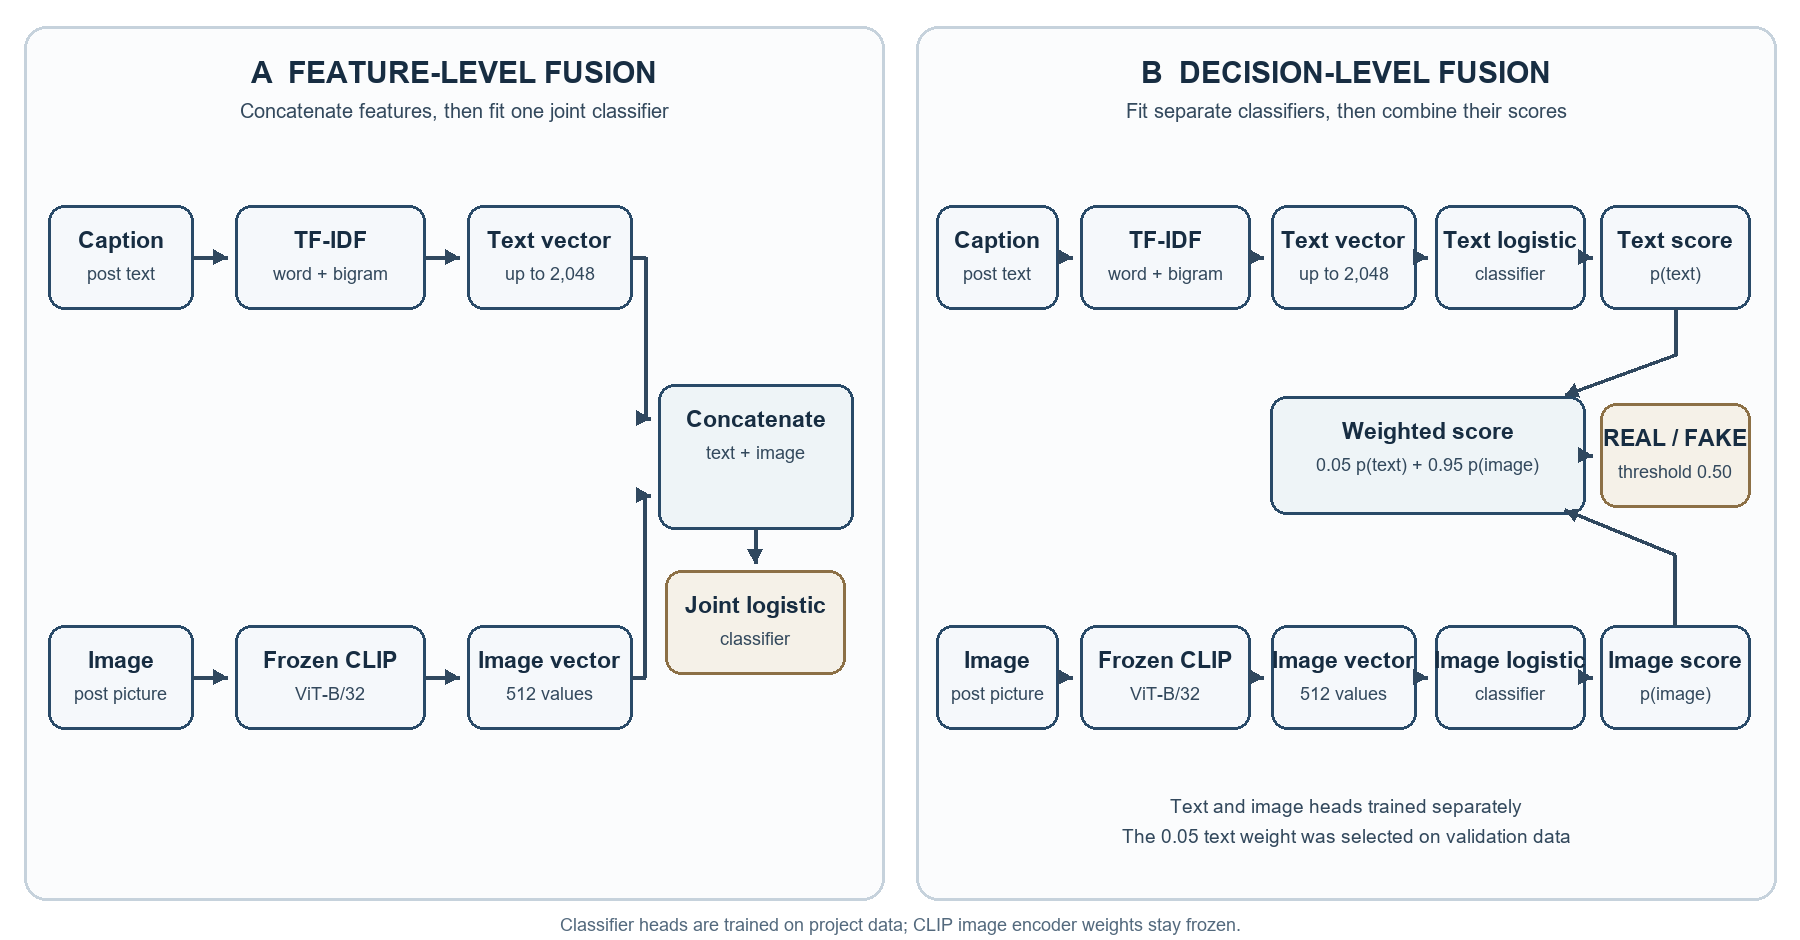
\includegraphics[width=0.94\textwidth]{architecture.png}
\caption{Real-media image-text architectures. Panel A concatenates TF-IDF text and frozen CLIP image features before a joint logistic classifier. Panel B fits separate text and image logistic heads, then combines their scores using validation-selected weights.}
\label{fig:real_architecture}
\end{figure*}
\subsection{Synthetic modality models}
The synthetic text branch lowercases and tokenizes captions, then constructs unigram and adjacent-bigram TF-IDF features using training captions only. The fitted vocabulary has 93 features. The image branch extracts 15 pixel-derived features, including foreground color, shape, object count, and simple component statistics. Each modality has its own L2-regularized logistic classifier.

Feature fusion concatenates both feature vectors with six explicit comparison features: color, shape, and count contradiction; contradiction fraction; all-attributes-match; and known-attribute fraction. The resulting model has 114 features. This design exposes the relation used to create labels. Decision-level fusion instead blends independent modality scores, with the weight selected by validation log loss. Vocabulary fitting, scaling, and classifier fitting do not use test labels.

The text branch is intentionally a compact baseline. For a token $t$ in document $d$, TF-IDF weights a term-frequency value by an inverse-document-frequency value estimated from the training corpus \cite{salton}. The vocabulary is then applied without refitting to validation and test captions. The synthetic branch learns a 93-feature vocabulary from its own training split; the real branch allows at most 2,048 word and adjacent-bigram features, uses sublinear term frequency, and discards terms occurring in fewer than two training documents. These settings reduce vocabulary leakage and keep the real text model independent from the image encoder.

Each classifier maps a feature vector $x$ to a class score through logistic regression. In the binary case, the estimated class score is computed with the logistic function applied to a linear combination of the input features. The coefficient vector and intercept are learned from the corresponding training partition using L2 regularization. Regularization controls the magnitude of the fitted weights. For feature fusion, $x$ contains the concatenated modality features and, for the synthetic profile, the explicit cross-modal comparison vector. For decision fusion, separate probabilities are combined after each modality model has been fitted; this does not allow one branch's representation to change during the other's optimization.

The six synthetic comparison features encode whether the caption and detected scene disagree on color, shape, and count; the fraction of those attributes that disagree; whether all known attributes match; and the proportion of attributes that can be compared. The image representation includes foreground color, shape, object count, foreground fraction, fill, and RGB/component statistics. This branch is based on image pixels and simple connected-object measurements. It is not the CLIP model. In the real-data profile, the frozen CLIP ViT-B/32 vision encoder maps an image to a normalized 512-dimensional representation, and a separately fitted logistic head maps that representation to a dataset label.
\subsection{Real-media modality models}
For real captions, a word-and-bigram TF-IDF vocabulary is fitted on training posts only, with at most 2,048 features, sublinear term frequency, and minimum document frequency two. An L2 logistic regression model is trained on these vectors. Regularization is selected by validation log loss.

For images, frozen CLIP ViT-B/32 produces normalized 512-dimensional visual features \cite{radford}. A separate L2 logistic head is trained on these features; CLIP weights are not fine-tuned. Feature fusion concatenates the visual and TF-IDF vectors and fits a third logistic head. Decision-level fusion combines text and image probabilities using a validation-selected text weight of 0.05. Standardization and fitting use training data; validation selects settings; test records are excluded from selection. The validation-selected real-data decision-fusion weight assigns 0.05 to the text score. The default classification threshold for reported binary predictions is 0.5. This separation is important: a held-out test score is meaningful only if the test labels do not influence vocabulary fitting, feature scaling, regularization selection, or fusion weights.

The evaluation reports accuracy, class-specific precision, recall, and F1, macro F1, ROC-AUC, average precision, and log loss where available. Accuracy is the fraction of all predictions that are correct. Precision and recall are calculated for the FAKE class unless a class is explicitly named; macro F1 averages the two class F1 values equally. ROC-AUC measures ranking across thresholds, while average precision summarizes the precision-recall curve and is affected by the positive-class prevalence. Log loss evaluates probability assignments and penalizes confident errors. None of these values is a calibration guarantee. The reported probabilities are model scores for dataset labels, not confidence that a claim is true or false.

The evaluation follows a partitioned training protocol. Training records fit the TF-IDF vocabulary, inverse document frequencies, any standardization parameters, and classifier coefficients. Validation records select regularization strength and the decision-level blend; the real-media validation log loss is also used to select the recommended model. The test partition is evaluated once after this selection. The synthetic in-distribution test and count-manipulation test remain separate from the real-media evaluation. No joint training or shared vocabulary is used across synthetic and real records, because such pooling would change both the data distribution and label definition.

For the real-data feature-fusion model, concatenation creates one vector with text and image features, after which a logistic classifier learns a joint linear decision surface. This is an early or feature-level fusion design. Late or decision-level fusion keeps the text and image classifiers independent and combines their output scores. Its text coefficient is selected on validation data and fixed before the final test run. Comparing these strategies helps distinguish whether a gain comes from joint representation fitting or merely averaging already trained predictions. In this run, feature fusion outperformed late fusion on accuracy, macro F1, ROC-AUC, and log loss, but the result is a single split estimate and does not prove universal superiority of feature fusion.

The synthetic and real text models use the same general TF-IDF-plus-logistic approach but are separately fitted. Their vocabularies, parameters, and targets are not shared. The synthetic label encodes constructed caption-scene agreement; the real label is an inherited source category. Pooling them would obscure that distinction.
\section{Experimental Results}
\subsection{Synthetic evaluation}
On the balanced 144-pair in-distribution test set, synthetic feature fusion achieves 1.000 accuracy and F1. The text-only baseline obtains 0.479 accuracy and 0.476 F1; the image-only baseline obtains 0.507 accuracy and 0.548 F1. Decision fusion matches the image branch in this run.

Table II summarizes the in-distribution synthetic test. The paired test includes 72 matching and 72 contradictory examples. The feature-fusion model recovers every label, while both unimodal baselines remain close to chance. This gap is expected for the construction: neither the caption words nor the scene attributes alone are sufficient to determine whether the pair agrees. The text-only classifier can learn correlations between wording and labels, and the image-only classifier can learn image-side correlations, but the decisive signal is whether the attributes correspond across modalities. The table does not imply that a 100 percent score is attainable on unconstrained image-caption data. \begin{table}[t]
\caption{Synthetic In-Distribution Test Results}\label{tab:synth}\centering\footnotesize
\begin{tabular}{lrrrr}
\hline Model & Acc. & Precision & Recall & F1\\\hline
Text-only TF-IDF + LR & 0.479 & 0.479 & 0.472 & 0.476\\
Image attributes + LR & 0.507 & 0.506 & 0.597 & 0.548\\
Feature fusion & 1.000 & 1.000 & 1.000 & 1.000\\
Decision fusion & 0.507 & 0.506 & 0.597 & 0.548\\\hline
\end{tabular}
\end{table}

On the count-manipulation test, feature fusion again obtains 1.000 accuracy and F1. This result is specific to the generated domain: explicit attribute comparisons closely match the rule used to create the labels. It is not evidence of equivalent performance on natural photographs.

The unimodal confusion matrices reinforce the role of cross-modal evidence. Text-only produced 35 true negatives, 37 false positives, 38 false negatives, and 34 true positives; image-only produced 30, 42, 29, and 43, respectively. The feature-fusion confusion matrix was perfect at 72 true negatives and 72 true positives. Decision-level fusion reproduced the image-only confusion matrix for this run. When the trained fusion model was evaluated with feature families replaced by their training means, removing cross-modal features returned accuracy and F1 to 0.500. Removing text gave 0.486 accuracy and 0.479 F1; removing the image features gave 0.465 accuracy and 0.476 F1. These are inference-time ablations of the fixed model, not newly trained leave-one-modality-out systems, so they show dependence of this model's predictions rather than the best possible single-modality performance.

The count test contains 72 REAL and 72 FAKE examples and produces 72 correct predictions in each class. Text-only and decision fusion each achieve approximately chance-level accuracy on this held-out contradiction type, and image-only achieves 0.500 accuracy with 0.539 F1. The fused classifier's perfect score is consistent with its access to the explicit count comparison.

The held-out count evaluation is particularly sensitive to feature design. The training task includes other contradiction types and the count-specific test uses unseen scene groups, but the captions and rendered objects still follow the same finite grammar. A rule-based extractor can identify number words and object counts consistently in this constrained setting. Consequently, success on this test demonstrates that the count comparison generalizes across generated scenes; it does not test robustness to pluralization errors, dense images, partially visible objects, or captions that imply counts indirectly. Future work should replace the generator with realistic examples and independently annotated agreement labels before making claims about practical image-text verification. Since count and other object attributes are readily parsed from the generator's captions and rendered pixels, this test probes transfer to a reserved mismatch type inside the same synthetic grammar, not transfer to an unseen visual domain.
\subsection{Real-media evaluation}
Table~\ref{tab:real} reports real-media test results at a fixed 0.5 threshold. Feature fusion achieves the best accuracy, macro F1, and ROC-AUC among the evaluated models. It improves over the unimodal baselines on these measures. Decision fusion does not improve over the individual models.
\begin{table}[t]
\caption{Real-Media Held-Out Test Results}\label{tab:real}\centering\footnotesize
\begin{tabular}{lrrrr}
\hline Model & Acc. & F1-FAKE & Macro F1 & AUC\\\hline
Majority baseline & 0.804 & 0.891 & 0.446 & 0.500\\
Text TF-IDF + LR & 0.818 & 0.896 & 0.571 & 0.742\\
Image CLIP + LR & 0.809 & 0.891 & 0.541 & 0.822\\
Feature fusion & \textbf{0.834} & \textbf{0.904} & \textbf{0.645} & \textbf{0.852}\\
Decision fusion & 0.807 & 0.891 & 0.528 & 0.827\\\hline
\end{tabular}
\end{table}
Accuracy alone hides difficulty with the minority REAL class. For feature fusion, REAL recall is 0.266, compared with FAKE recall of 0.973. The training-majority baseline already reaches 0.804 accuracy by predicting FAKE for every test record. The fusion model's gain in accuracy is modest; its higher macro F1 and ROC-AUC add information but do not remove imbalance or label-quality concerns. The explicitly manipulated-content category is rare in the test partition, so this experiment does not validate pixel-level manipulation detection.

The confusion counts for the real-media models are shown in Table IV. TN, FP, FN, and TP treat FAKE as the positive class; rows are source REAL and FAKE labels, and the threshold is fixed at 0.5.
\begin{table}[t]
\caption{Real-Media Confusion Counts}\label{tab:conf}\centering\footnotesize
\begin{tabular}{lrrrr}
\hline Model & TN & FP & FN & TP\\\hline
Text-only & 42 & 236 & 22 & 1,115\\
Image-only & 32 & 246 & 25 & 1,112\\
Feature fusion & 74 & 204 & 31 & 1,106\\
Decision fusion & 27 & 251 & 22 & 1,115\\\hline
\end{tabular}
\end{table}

The counts show that fusion's improvement is concentrated in identifying more REAL examples at this threshold. Relative to text-only, it correctly predicts 32 additional REAL examples but also makes nine additional errors on FAKE examples. Relative to image-only, it increases correct predictions for both classes in this partition. These are descriptive differences for the same held-out examples, not evidence of statistical significance. They do not reveal whether a post's source label is itself correct, nor do they show whether the model relies on semantic evidence or dataset correlations. The counts complement the aggregate table by making the class-specific tradeoff directly inspectable.

At the fixed threshold, feature fusion has the confusion matrix $[[74,204],[31,1106]]$ with true and predicted labels ordered REAL then FAKE. It correctly identifies 74 of 278 REAL examples and 1,106 of 1,137 FAKE examples. The corresponding recalls are 0.2662 and 0.9727. REAL precision is 0.7048 and REAL F1 is 0.3864; FAKE precision is 0.8443 and FAKE F1 is 0.9040. The balanced accuracy, the arithmetic mean of the two recalls, is 0.6195.
\begin{table}[t]
\caption{Feature-Fusion Test Results by Class}\label{tab:class}\centering\footnotesize
\begin{tabular}{lrrrr}
\hline Class & Precision & Recall & F1 & Support\\\hline
REAL & 0.7048 & 0.2662 & 0.3864 & 278\\
FAKE & 0.8443 & 0.9727 & 0.9040 & 1,137\\\hline
\end{tabular}
\end{table}
 The baseline predicts no REAL examples, so its REAL recall is zero even though its accuracy is 0.8035. This is why a small accuracy improvement should not be described as balanced detection.

Feature fusion also has average precision 0.9587 and log loss 0.3609, compared with 0.9130 and 0.4318 for text-only, and 0.9519 and 0.3882 for image-only. The late-fusion model reaches 0.9534 average precision and 0.3867 log loss. These probability and ranking metrics favor feature fusion in this one held-out partition, but the high prevalence of FAKE contributes to the precision-recall results. A threshold selected for a different operating cost could alter precision and recall substantially. The threshold of 0.5 was kept fixed for the reported class metrics; no claim is made that it is optimal for deployment.
\subsection{Interpretation}
The datasets support different conclusions. In the synthetic task, either caption or image alone is weak because labels depend on a relation between modalities; explicit comparisons make that relation available to fusion. In the real-media subset, independent TF-IDF text and CLIP image branches predict inherited labels, and feature fusion improves held-out ranking and macro F1. Weak labels, uncertain split provenance, possible near-duplicates, and unknown pretraining overlap limit interpretation. Probabilities are uncalibrated dataset scores. No independent-domain evaluation, human explanation study, or real-world fact verification was performed.

The interpretation of fusion gains should also consider confounding. A fused classifier can exploit correlations between text, image, and inherited label that do not represent semantic agreement. A source community's topic or style can correlate with the class; an image can also be associated with a topic without directly supporting a caption. The source and mirror documentation are insufficient to determine how much such shortcuts contribute. The synthetic benchmark avoids these open-world label questions but introduces a simpler shortcut: its six explicit comparisons are closely aligned with the exact way contradictions are generated. Both experiments are informative when stated narrowly, and neither alone establishes robust multimodal reasoning.

A low-margin review was also performed on the synthetic test set by selecting eight examples from each class after model fitting. The reviewed examples were not necessarily errors; they were the closest predictions to the decision boundary among the selected records. The recorded cases were correctly classified, and the reported false-caption examples had a visible color or shape contradiction while the matching REAL examples agreed on color, shape, and count. For example, a caption describing a yellow square paired with a green square was identified through a color conflict. This illustrates how the controlled feature representation supports a direct attribute-based account of a prediction. However, the selected examples still had high model scores, and the review set was small and chosen from the same synthetic test partition. It is therefore a qualitative sanity check, not a general error analysis or a human evaluation.

The perturbation analysis provides a limited diagnostic for that narrow synthetic setting. Token deletion changes are evaluated while keeping the image fixed, and counterfactual caption edits test whether the score moves in the expected direction. Because these modifications are selected to alter known attributes, the observed response is a consistency check on the implemented cues. It does not establish causal feature importance across arbitrary examples. Similarly, masking detected object regions can alter an input beyond the training distribution, so any score change from occlusion should be interpreted cautiously. No human raters judged the explanations, and the real-media classifier's explanations were not validated in this project.

This distinction also limits interpretation of a high FAKE probability. The output estimates a model score for the mapped source class and may be driven by words, visual subject matter, or dataset artifacts. It does not measure author intent, the truth of a claim, or whether an image has been altered. In particular, the source taxonomy's manipulated category is only one part of FAKE and is rare in this subset; overall binary metrics cannot be read as a dedicated manipulation-detection result. The project's synthetic explanations describe generated attribute contradictions, while no equivalent human-validated explanation is available for arbitrary real posts.

A perturbation analysis was recorded only for the synthetic model. On a fixed set of 48 test records, removing attribute-bearing caption tokens changed the FAKE score more than removing filler tokens: the mean absolute effects were 0.2859 and 0.0006, respectively. Correcting false captions reduced the FAKE score by 0.9239 on average, while adding a color contradiction to matching captions increased it by 0.9268 on average; the expected direction was observed for all tested cases. These checks indicate sensitivity to the intended lexical and attribute cues. They are local input perturbations, not causal explanations, and the evaluation did not include a human assessment of whether a rationale was useful or faithful for natural posts.
The study also has several reproducibility constraints. For the real profile, the data mirror revision is pinned to \texttt{2ba956a67d2bab34de97b25d71af520ab3fe1e6e}, and the feature extractor revision recorded in the project artifacts is \texttt{3d74acf9a28c67741b2f4f2ea7635f0aaf6f0268}. A manifest checksum, duplicate-audit outputs, and run summaries are retained with the repository. The real training entry point is \texttt{scripts/train\_real.py}; the synthetic generation and experiment entry points are \texttt{scripts/generate\_dataset.py} and \texttt{scripts/run\_experiments.py}. Reproduction requires the prepared local data and encoder files documented by the project. These records allow a reader to identify the intended inputs and rerun model fitting, but they cannot recover missing Reddit post identifiers or reconstruct undocumented sampling decisions in the mirror.

The evaluation is also limited to one fixed partition for each profile. Validation avoids test-label selection for the model settings, but the report does not provide confidence intervals, repeated random splits, or a separate external test corpus. Near duplicates that are not captured by the available identifiers may remain. The frozen visual encoder's full pretraining corpus is not auditable from the local experiment, so pretraining overlap cannot be excluded. Finally, real-media outputs have not been evaluated for calibration, human explanation quality, or utility in a review workflow. These boundaries are material to interpreting the reported measurements and should be addressed before the system is used beyond this course project.

\section{Conclusion and Future Work}
VeriFuse implements modality-specific text and image models and evaluates them on a controlled synthetic benchmark and a separate real-media subset. Synthetic feature fusion scores perfectly on held-out splits, while unimodal classifiers remain near chance; this measures the implemented consistency rule. On the real-media test set, TF-IDF text classification reaches 0.818 accuracy and CLIP-image classification reaches 0.809; feature fusion raises accuracy to 0.834 and macro F1 to 0.645. The real-media result remains constrained by imbalance and inherited labels, including low REAL recall.

Taken together, the two profiles show why modality-specific models must be evaluated against task-specific targets. The synthetic experiment provides a transparent test of whether designed scene attributes and caption attributes agree. The real-media experiment offers a more realistic distribution of images and text but weaker target validity because its labels come from source categories. Their scores are therefore reported independently. A strong synthetic result cannot compensate for limited real-label validity, and a better ranking score on the mirror does not prove that the model recognizes semantic contradiction. The most defensible conclusion is narrower: explicit comparisons solve the generated rule, and concatenated TF-IDF/CLIP features improve several held-out metrics for this mirror's binary label mapping.

Future work should validate the real branch on an independently sourced and documented dataset with event-level splits and stronger class balance. The next evaluation should record the original post and event identifiers, audit near duplicates across partitions, and document how sampling and labels were produced. If the goal is factuality rather than source-label classification, labels should be independently verified for the relevant claim and image-text relation. Results should be reported separately for satire, false connection, imposter, manipulated, and misleading categories before deciding whether those distinct targets should be combined.

Threshold selection should account for false-positive and false-negative costs, and probability calibration should be measured on held-out data. The image branch needs evaluation on a dedicated manipulation benchmark before any authenticity claim. A separately trained or fine-tuned language model could replace TF-IDF in a future controlled comparison; the present results do not establish that it would improve performance. Further experiments should compare frozen and fine-tuned visual encoders under the same data split, use repeated group-aware validation where feasible, and test the final system on an external corpus. Error analysis should include the minority REAL class and should distinguish source-label ambiguity from actual model mistakes. For any user-facing deployment, uncertain or high-impact cases should be escalated to human review rather than treated as verified truth.
\begin{thebibliography}{00}
\bibitem{nakamura} K. Nakamura, S. Levy, and W. Y. Wang, \textquotedblleft Fakeddit: A new multimodal benchmark dataset for fine-grained fake news detection,\textquotedblright in \textit{Proc. LREC}, 2020, pp. 6149--6157.
\bibitem{radford} A. Radford \textit{et al.}, \textquotedblleft Learning transferable visual models from natural language supervision,\textquotedblright in \textit{Proc. ICML}, 2021, pp. 8748--8763.
\bibitem{rossler} A. R\"ossler \textit{et al.}, \textquotedblleft FaceForensics++: Learning to detect manipulated facial images,\textquotedblright in \textit{Proc. IEEE/CVF ICCV}, 2019, pp. 1--7.
\bibitem{salton} G. Salton and C. Buckley, \textquotedblleft Term-weighting approaches in automatic text retrieval,\textquotedblright \textit{Information Processing \& Management}, vol. 24, no. 5, pp. 513--523, 1988.
\bibitem{labelmap} Entitize, \textquotedblleft Fakeddit label mapping clarification,\textquotedblright GitHub issue comment, 2021. [Online]. Available: \url{https://github.com/entitize/Fakeddit/issues/14#issuecomment-815355653}
\bibitem{mirror} ams-99, \textquotedblleft Fakeddit 9k community mirror,\textquotedblright Hugging Face Datasets, revision \texttt{2ba956a67d2bab34de97b25d71af520ab3fe1e6e}, 2026. [Online]. Available: \url{https://huggingface.co/datasets/ams-99/fakeddit\_9k}
\end{thebibliography}
\end{document}
